\subsection{Topic Specific PageRank} \label{sec:Topic specific PR}
Haveliwala suggested a pseudo-personalised PR algorithm known at Topic-Specific PageRank,TSPR, which aims to group users in order to lessen the computation of unique personalised PR for each user \cite{haveliwala2002topic}. This is done by biasing the PR vectors created to a set of representative topics \cite{haveliwala2002topic}, where the bias PR vectors are calculated prior to query time \cite{langville}, this biasing involves the introduction of artificial links into the web graph. The biases are applied during iterations to increase the importance of certain categories and pages \cite{haveliwala1999efficient}. The use of the TSPR generates more accurate ranking than the single generic PR vector, as a certain user will be more interested in some topics, and so intuitively these pages should have a higher ranking. 

TSPR is similar to HITS, as discussed in Section \ref{sec:HITS}, as it is a query-dependant algorithm, which allows the query to impact the ranking, however like PR there is minimal query-time processing. 

TSPR is also less vulnerable to topic drift, as we avoid the problem of heavily linked web pages having a high ranking for queries that they have little authority. 

TSPR suggests that the web page can be represented sufficiently by 16 main topics;
\begin{enumerate}
\item Arts
\item Business
\item Computers
\item Games
\item Health
\item Home
\item Kids \& teens
\item News
\item Recreation
\item Reference
\item Regional
\item Science
\item Shopping
\item Society
\item Sports
\item World
\end{enumerate} During the offline crawl, 16 TSPR vectors are created from information supplied by the user. This information can be created automatically from an analysis of the bookmarks and browser history over time, or the user could manually input their preference for each topic, the algorithm assumes that an individuals interest can be approximated sufficiently as a linear combination of the smaller topic page distributions \cite{manning}.
\begin{figure}[h!]
\centering
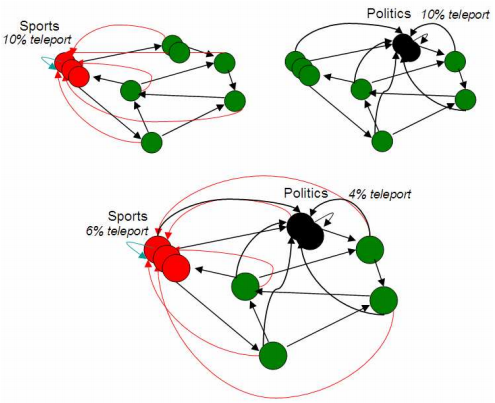
\includegraphics[width=10cm]{Topic-specific_PageRank_Manning.png}
\caption{Topic-specific PageRank, where a user has 60\% interest in sports, and 40\% interest in politics, taken from \cite{manning}}
\label{fig:topic-specific}
\end{figure}

In Figure \ref{fig:topic-specific}, $\alpha$ is 0.9, the user will teleport 6\% to sports pages, and 4\% to politics pages.

At query time, the algorithm calculated the similarity of the query (including the user context if available) to each of these topics, and then takes a linear combination of the TSPR vectors weighted with respect to the similarity of the query (and context) to the topic. As the computation of the TSPR is done prior to query-time, the algorithm doesn't have large query-time costs \cite{haveliwala2002topic}.  The TSPR vectors are denoted as $\boldsymbol{\pi}_t$ where \textit{t} denotes the topic, for example the sports PageRank vector would be $\boldsymbol{\pi}_s$, each user would have a mixture of interests, for example User P could be interested in sports 60\%, but also interested in politics 40\%, and so the TSPR would be $\boldsymbol{\pi}_P=0.6\pi_s+0.4\pi_p$, this would lead to a Markov chain with a steady state distribution that has been personalized. 


Forms a topic-sensitive, query-dependant PR vector which is a convex combination of PR vectors \cite{langville}. This uses a bayesian classifier in order to compute the $\beta_i$'s for the experiments \cite{langville}.   The implementation of TSPR is costly as for each user there is a need to compute a unique transition matrix \cite{manning}. 
